\setchapterimage[7.5cm]{images/daniel-sinoca-AANCLsb0sU0-unsplash}
\setchapterpreamble[u]{\margintoc}
\chapter{Unit (Component) Testing}
\section{Unit Testing Basics}
First level of testing is unit testing. Unit (component) is a manageable piece of code which may produce a result, perform a computation and return its result(s) to its caller, or may call some other function or method. In procedural programming, a unit could be an individual function or procedure (subroutine). In an object-oriented setting, a unit could be an individual method or even a class. 

Unit testing is a low-level testing technique by means of which individual units are tested to determine if they produce expected outcomes or not. All assignment statements and predicates (logical expressions) in the code must be run, as well as all paths, while achieving the expected output with the unit test. In general, unit testing activity can be described as a type of testing process used to verify and validate a specific unit of the code for its correctness to cover the coding standards, functionality, integration, code coverage, security features, compatibility, performance, and so on. Unit testing is done by the person who develops the unit. The following unit examples are written in C and Java.

\begin{example}
Write a C function \textbf{solveQuadratic} to solve the quadratic $ax^2+bx+c=0$ for the two real roots x1, and x2. Coefficients of the quadratic polynomial is to be provided by the calling program.

\begin{lstlisting}[language=C, caption={A C function that solves the quadratic equation for the two real roots.}]
double solveQuadratic(double a, double b, double c) {
	double disc, x1, x2;
	disc = b * b - 4.0 * a * c;
	if (disc < 0) {
		printf("Discriminant = %f7.4 :no real roots!", disc);
	} else {
		x1 = (-b + sqrt(disc) / (2.0 * a);
		x2 = (-b - sqrt(disc)) / (2.0 * a);
		printf("x1 = %f7.4, x2 = %f7.4\n",x1, x2);
	}
	return (0);
}
\end{lstlisting}
\end{example}


\begin{example}
\labexample{ex22}
Binary search is a very effective technique to search an element in a set of ordered elements stored in an array. The following C program is an implementation borrowed from \url{https://www.tutorialspoint.com/compile_c_online.php}. Some bugs are  intentionally inserted into the code. The reader is encouraged to review this example, identify and correct errors, and run it again. 
\begin{lstlisting}[language=C, caption={Binary search A C implementation.}]
// Iterative C Program for Binary Search (GNU GCC v7.1.1)
// Adapted from https://www.tutorialspoint.com/codingground.htm
// 3 severe bugs are inserted! 
#include <stdio.h>
int BinarySearch(int array[], int left, int right, int element){
   while (left <= right){
      int middle = left + (right + left)/2;
      if (array[middle] == element)
         return middle;
      if (array[middle] < element)
         left = middle - 1;
      else
         right = middle + 1;
   }
   return -1;
}
int main(void){
   int array[] = {11, 14, 17, 21, 28, 43, 41, 52, 56, 70, 76, 82, 99};
   int n = 13;
   int element = 99;
   int index = BinarySearch(array, 0, n-1, element);
   if(index == -1 ) {
      printf("Element not found!");
   }
   else {
      printf("Element found at position : %d",index);
   }
   return 0;
}
\end{lstlisting}
\end{example}
Unit testing is conducted in two different but complementary phases, namely, static unit testing and dynamic unit testing. In static unit testing, the unit under the test is examined, without actually executing it, to infer conclusions about its functionality, and causes of some possible faults. In dynamic unit testing, a program unit is actually executed and its outcomes are recorded and analysed.

\section{Static Unit Testing – Code Reviews}
Static unit testing\index{static unit testing} is accomplished by using several code review techniques. Code review is not restricted to units. In practice, during this process, completed parts of the code (unit, module, or component) are reviewed using inspection and walkthrough techniques. Inspection\index{inspection} is a step by step peer group review of a work product (including a document), with each step checked against predetermined criteria \autocite{fagan1999design}. Walkthrough\index{walkthrough} is a similar review technique in which the developer leads the team through a manual or simulated execution of the product using predefined scenarios \autocite{yourdon1989structured}. 

The main goal of the code review is to review the code in an attempt to find the errors in the code before it is passed on to another activity (e.g., integration testing). The code review should be performed in a systematic manner by executing planned activities. To facilitate the process a review team is established. Review team is usually made up of members who will assume the roles of facilitator, code developer (author), presenter, record keeper, reviewer, and observer.
The general guidelines for performing code review consists of six steps \autocite{naik2011software}.

\begin{description}
    \item[Readiness] Unit developer assures that the unit is ready for inspection. 
    \item[Preparation] Each reviewer goes over the code and the related documents. A list of potential CR is prepared by the reviewers.
    \item[Examination and Producing a Change Request (CR) Document] In this step, the author, presenter, the record keeper, and the moderator are involved and, if needed, a CR document is prepared and passed on to the next step.
    \item[Rework] The CR list that needs to be resolved is forwarded to the developer.
    \item[Validation] The rework done by the developer is validated by one of the software team members. The validation process involves checking the improvements in the code as suggested by the other group members. 
    \item[Reporting] If all CRs are fulfilled, a detailed report is prepared and shared with the team members.
\end{description}

To facilitate the code review process, software teams use predefined checklists. One such checklist is given below\sidenote[][-1.5cm]{This document\\\url{https://github.com/mgreiler/code-review-checklist} is protected under the MIT license}. 

\paragraph{Implementation}
\begin{enumerate}
    \item Does this code change do what it is supposed to do?
    \item Can this solution be simplified?
    \item Does this change add unwanted compile-time or run-time dependencies?
    \item Was a framework, API, library, service used that should not be used?
    \item Was a framework, API, library, service not used that could improve the solution?
    \item Is the code at the right abstraction level?
    \item Is the code modular enough?
    \item Would you have solved the problem in a different way that is substantially better in terms of the code’s maintainability, readability, performance, security?
    \item Does similar functionality already exist in the codebase? If so, why isn't this functionality reused?
    \item Are there any best practices, design patterns, or language-specific patterns that could substantially improve this code?
    \item Does this code follow Object-Oriented Analysis and Design Principles, like the Single Responsibility Principle, Open-close principle, Liskov Substitution Principle, Interface Segregation, Dependency Injection?
\end{enumerate}

\paragraph{Logic Errors and Bugs}
\begin{enumerate}
  \setcounter{enumi}{11}
  \item Can you think of any use case in which the code does not behave as intended?
  \item Can you think of any inputs or external events that could break the code?
\end{enumerate}
 
\paragraph{Error Handling and Logging} 
\begin{enumerate}
  \setcounter{enumi}{13}
  \item Is error handling done the correct way?
  \item Should any logging or debugging information be added or removed?
  \item Are error messages user-friendly?
  \item Are there enough log events and are they written in a way that allows for easy debugging?
\end{enumerate}

\paragraph{Usability and Accessibility}
\begin{enumerate}
 \setcounter{enumi}{17}
  \item Is the proposed solution well designed from a usability perspective?
  \item Is the API well documented?
  \item Is the proposed solution (UI) accessible?
  \item Is the API/UI intuitive to use?
\end{enumerate}
 
\paragraph{Ethics and Morality}
\begin{enumerate}
 \setcounter{enumi}{21}
 \item Does this change make use of user data in a way that might raise privacy concerns?
 \item Does the change exploit behavioral patterns or human weaknesses?
 \item Might the code, or what it enables, lead to mental and physical harm for (some) users?
 \item If the code adds or alters ways in which people interact with each other, are appropriate measures in place to prevent/limit/report harassment or abuse?
 \item Does this change lead to an exclusion of a certain group of people or users?
 \item Does this code change introduce any algorithm, AI or machine learning bias?
 \item Does this code change introduce any gender/racial/political/religious/ableist bias?
\end{enumerate}
 
\paragraph{Testing and Testability}
\begin{enumerate}
 \setcounter{enumi}{28}
 \item Is the code testable?
 \item Does it have enough automated tests (unit/integration/system tests)?
 \item Do the existing tests reasonably cover the code change?
 \item Are there some test cases, input, or edge cases that should be tested in addition?
\end{enumerate}
 
\paragraph{Dependencies} 
\begin{enumerate}
 \setcounter{enumi}{32}
  \item If this change requires updates outside of the code, like updating the documentation, configuration, readme files, was this done?
  \item Might this change have any ramifications for other parts of the system, backward compatibility?
\end{enumerate}

\paragraph{Security and Data Privacy}
\begin{enumerate}
 \setcounter{enumi}{34}
  \item Does this code open the software for security vulnerabilities?
  \item Are authorization and authentication handled in the right way?
  \item Is sensitive data like user data, credit card information securely handled and stored? Is the right encryption used?
  \item Does this code change reveal some secret information (like keys, usernames, etc.)?
  \item If code deals with user input, does it address security vulnerabilities such as cross-site scripting, SQL injection, does it do input sanitization and validation?
  \item Is data retrieved from external APIs or libraries checked accordingly?
\end{enumerate}

\paragraph{Performance}
\begin{enumerate}
 \setcounter{enumi}{40}
  \item Do you think this code change will impact system performance in a negative way?
  \item Do you see any potential to improve the performance of the code?
  \end{enumerate}
	
\paragraph{Readability}
\begin{enumerate}
 \setcounter{enumi}{42}
   \item Was the code easy to understand?
   \item Which parts were confusing to you and why?
   \item Can the readability of the code be improved by smaller methods?
   \item Can the readability of the code be improved by different function/method or variable names?
   \item Is the code located in the right file/folder/package?
   \item Do you think certain methods should be restructured to have a more intuitive control flow?
   \item Is the data flow understandable?
   \item Are there redundant comments?
   \item Could some comments convey the message better?
   \item Would more comments make the code more understandable?
   \item Could some comments be removed by making the code itself more readable?
    \item Is there any commented out code?
\end{enumerate}

\paragraph{Experts Opinion}
\begin{enumerate}
 \setcounter{enumi}{54}
   \item Do you think a specific expert, like a security expert or a usability expert, should look over the code before it can be committed?
   \item Will this code change impact different teams? Should they have a say on the change as well? 
\end{enumerate}

The code review checklist list above is comprehensive enough to be used at different levels of testing. However, for unit testing, it would be more appropriate to use a modified and shortened version of the list.

\section{Dynamic Unit Testing}
In dynamic unit testing\index{dynamic unit testing}, the unit under investigation is executed in order to detect the errors. An execution environment is created by writing a test driver\index{test driver} and compiling it together with the actual unit. If the unit under the test invokes (calls) some other units, dummy ones called stubs\index{stubs} are created to emulate the called units.

\marginnote[-5cm]{
	\begin{kaobox}[frametitle=Test Driver]
    A test driver is simply a program (main) that calls the unit under test. Test input data is provided by the test driver, unit is called, and the results are returned from the unit and assessed (test fails/passes) by the test driver.
    \end{kaobox}
}

It is important to note that, the test driver and the stubs are retained and reused in the future in regression testings if required. In \reffig{fig:unit-env}, a dynamic unit testing environment is illustrated.

\marginnote{
	\begin{kaobox}[frametitle=Stub]
    A stub as mentioned before, is a dummy function which replaces the actual unit called by the unit under test. A stub returns a preassigned or decided value (e.g., null, 0, or another expected result from the actual unit) so that the unit under test can resume its execution in a meaningful way.
    \end{kaobox}
}

\begin{figure}[!ht]
    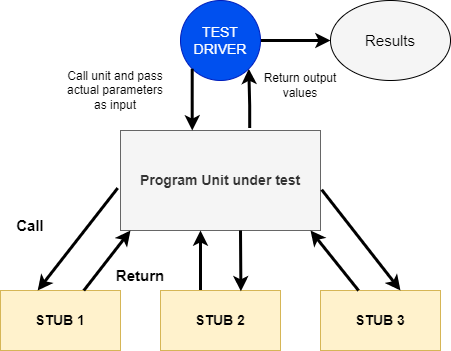
\includegraphics{images/unit-env.png}
    \caption{Validation and verification with the V-model.}
    \labfig{fig:unit-env}
\end{figure}

Test case generation (manual or automatic) is one of the main issues of software testing research. In unit testing, the main concern is to detect the faults (bugs) in the assignment and control statements, predicates (logical expressions in the control statements), and the flow of data from one statement to another. Test input selection is mainly based on Control Flow Testing, Data Flow Testing, and Functional Program Testing techniques. These techniques will be discussed in the chapters to follow. 

\section{Mutation Testing}
Mutation testing is a white-box testing technique to measure the adequacy of test cases \autocite{demillo1978hints}. The idea in mutation testing\index{mutation testing} is to test the code by modifying/altering the program intentionally by applying one of the there mutation types, and observe how the code behaves when tested with the same test data.  Each modified code is known as a mutant.

There are three types of mutation:
\begin{description}
    \item[Value mutation] Change one constant to a larger value or to a smaller value.
    \item[Statement mutation] Change the statements by removing/deleting or modifying the line.
    \item[Decision mutation] Change the decisions/conditions to check for the design errors. Typically, one changes the arithmetic operators (e.g., -, +, /, *) and mutating all relational operators (==, !=, <, <=, >, >=) and logical operators (AND, OR , NOT)).
\end{description}
A mutant is said to be killed if the execution of a test case causes it to fail. Some mutants are equivalent to the given program producing the same output as the original one. The mutants still alive are survived mutants and need to be killed by adding additional tests to the test suite. A mutation score, MS, for a set of test cases is defined as the percentage of nonequivalent mutants killed by the test suite. If K is the number of killed mutants, N is the total number of mutants, and E is the number of equivalent mutants, then $MS = \frac{k}{N - E} * 100\%$. The test suite is mutation adequate if the mutation score is 100\%. . 
\begin{example}
The following recursive C program prints the factorial of integers from 0 to 10. Create two mutants by applying value, and decision mutations and compute the mutation score.

\begin{lstlisting}[language=C, caption={A recursive C program to compute and print  0!, 1!,\ldots,10!}]
#include <stdio.h>
int fact (int);

main(){
	int k;
	for(k = 0; k <= 10; k++)
		printf("%2d! = %4d\n", k, fact(k));
}
int fact(int num){
	if (num <= 1)
		return (1);
	else
		return(num * fact(num - 1));
}
\end{lstlisting}
Output is a list of factorial values of numbers from 0 to 10.
\begin{lstlisting}[language=C, caption={Mutant 1: (Decision mutation - Change num <= 1 to num < 1)}]
#include <stdio.h>
int fact (int);

main(){
	int k;
	for(k = 0; k <= 10; k++)
		printf("%2d! = %4d\n", k, fact(k));
}
int fact(int num){
	if (num >= 1)
		return (1);
	else
		return(num * fact(num - 1));
}
\end{lstlisting}
\begin{lstlisting}[language=C, caption={Mutant 2: (Value mutation - Change fact(num –  1) to fact(num  - 100))}]
#include <stdio.h>
int fact (int);

main(){
	int k;
	for(k = 0; k <= 10; k++)
	printf("%2d! = %4d\n", k, fact(k));
}
int fact(int num){
	if (num <= 1)
		return (1);
	else
		return(num * fact(num - 100));
}
\end{lstlisting}
\begin{lstlisting}[language=C, caption={Mutant 3: (Decision mutant – Change  if (num <= 1) to if (num < 1))}]
#include <stdio.h>
int fact (int);

main(){
	int k;
	for(k = 0; k <= 10; k++)
	printf("%2d! = %4d\n", k, fact(k));
}
int fact(int num){
	if (num < 1)
		return (1);
	else
		return(num * fact(num - 1));
}
\end{lstlisting}
For the example above the test suite consists of 3 test cases:

\begin{itemize}
    \item Test case 1: <no input, error message >
    \item Test case 2: <no input, <1, 2, 3, 4, 5, 6, 7, 8, 9, 10> > (result is incorrect!)
    \item Test case 3: <no input, correct result>
\end{itemize}

Test case 1, and Test case 2 fail and therefore said to be killed by these test cases ($K=2$). However, Test case 3 produces correct result (factorial of numbers from 0 to 10 are printed correctly!) and is considered as an equivalent mutant ($E=1$). The mutation score in this case is $\frac{2}{3 - 1} * 100 = 100\%$.
\end{example}

\begin{example}
The following C program prints the prime numbers from 2 to n, where the value of n is the input. Create three mutants by applying value, and decision mutations and compute the mutation score.

\begin{lstlisting}[language=C, caption={A C program to compute and print primes from 2 to $n$.}]
//Prime numbers from 2 to n
#include<stdio.h>
main()
	printf("Enter the value of n>=2:\n");
	scanf("%d",&n);
	printf("Prime numbers are\n"); 
	for(i=2;i<=n;i++){
		int k=0;
		for(j=1;j<=i;j++)
			if(i%j==0)k++;		
		if(k==2)
			printf("%d ",i);
	}	
}
\end{lstlisting}
\begin{lstlisting}[language=C, caption={Mutant 1: (Decision mutant – Change $i \leq n$ to $i \geq n$)}]
//Prime numbers from 2 to n
#include<stdio.h>
main(){
	int i,j,n;
	printf("Enter the value of n>=2:\n");
	scanf("%d",&n);
	printf("Prime numbers are\n"); 
	for(i=2;i>=n;i++){
		int k=0;
		for(j=1;j<=i;j++)
			if(i%j==0)k++;		
		if(k==2)
		printf("%d ",i);
	}	
}
\end{lstlisting}
\begin{lstlisting}[language=C, caption={Mutant 2: (Decision mutant – Change $i \leq n$ to $i < n$)}]
//Prime numbers from 2 to n
#include<stdio.h>
main(){
	int i,j,n;
	printf("Enter the value of n>=2:\n");
	scanf("%d",&n);
	printf("Prime numbers are\n"); 
	for(i=2;i<n;i++){
		int k=0;
		for(j=1;j<=i;j++)
			if(i%j==0)k++;		
		if(k==2)
			printf("%d ",i);
	}	
}
\end{lstlisting}
\begin{lstlisting}[language=C, caption={Mutant 3: (Value mutant – Change $k == 2$ to $k == 3$)}]
//Prime numbers from 2 to n
#include<stdio.h>
main(){
	int i,j,n;
	printf("Enter the value of n>=2:\n");
	scanf("%d",&n);
	printf("Prime numbers are\n"); 
	for(i=2;i<=n;i++){
		int k=0;
		for(j=1;j<=i;j++)
			if(i%j!=0)k++;		
		if(k==3)
			printf("%d ",i);
	}	
}
\end{lstlisting}
For an input value of 19 for n, the original program produces the primes correctly from 2 to 19.

Output: 2, 3, 5, 7, 11, 13, 17, 19

Three test cases are as follows:
\begin{itemize}
    \item Test case 1: <19, null > Test fails! No primes are generated. 
    \item Test case 2: <19, <2, 3, 5, 7, 11, 17> > Test fails! 19 is missing from the list of primes.
    \item Test case 3: <19, 5> Test fails! Only one prime number, 5, is generated.
\end{itemize}
All tests fail, and there are no equivalent mutants. The mutation score in this case is  $\frac{3}{3} * 100 = 100\%$.
\end{example}

\section{Debugging}
Debugging\index{debugging} is a systematic process of finding and fixing the number of faults (bugs), or defects, in a piece of code so that the software is behaving as expected. For small to medium size software, developers can use brute force approach to find faults by inserting print statements in the neighborhood of the possible fault(s). For large size projects this approach is so tedious and therefore the use dynamic debuggers provided in the Integrated Development Environments (IDEs) should be utilized. A screenshot from Dev-\CC IDE debugger of a program is shown in \reffig{fig:devcpp-debugger}. Breakpoints are placed at certain lines (red color), and the change in the values of a variable is observed by adding a watch. Next line tab takes the execution to the next statement and the changes are observed on the Debug tab of the IDE.

\begin{figure}[!ht]
    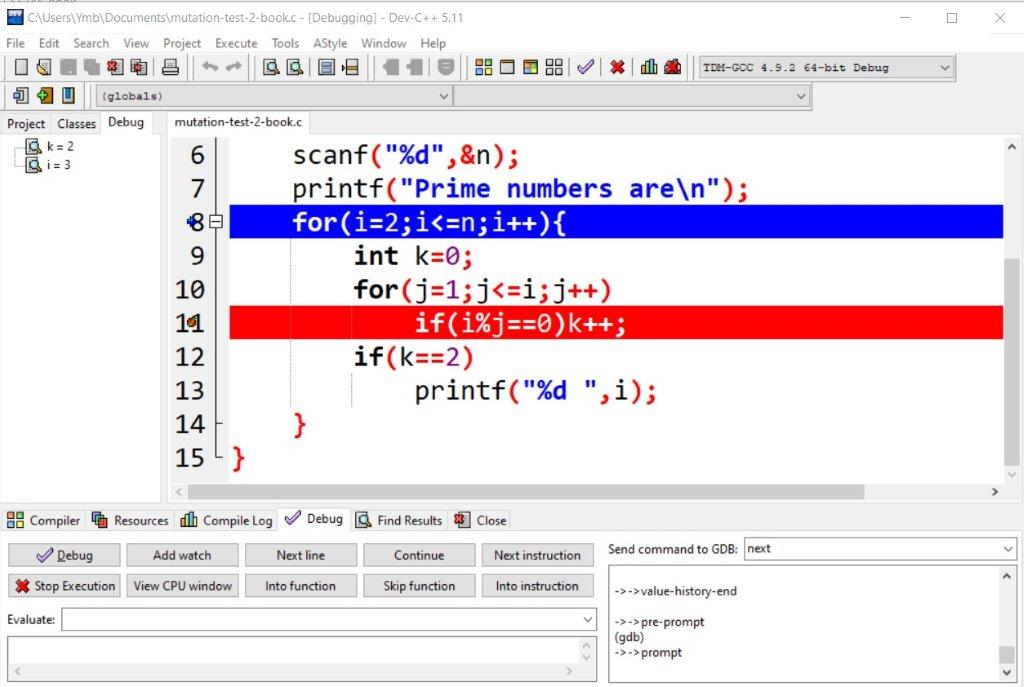
\includegraphics{images/dev-c-debugger.jpg}
    \caption{A screenshot of Dev-\CC Debugger.}
    \labfig{fig:devcpp-debugger}
\end{figure}
 
The reader is encouraged to learn the use of the debugger on DEV-\CC IDE by running and debugging the prime number generation program given above. Eclipse Java IDE used in the laboratory sessions, also offers similar debugging functionality. A screenshot from the debugging option of the Eclipse can be found in \reffig{fig:eclipse-debugger}.

\begin{figure}[!ht]
    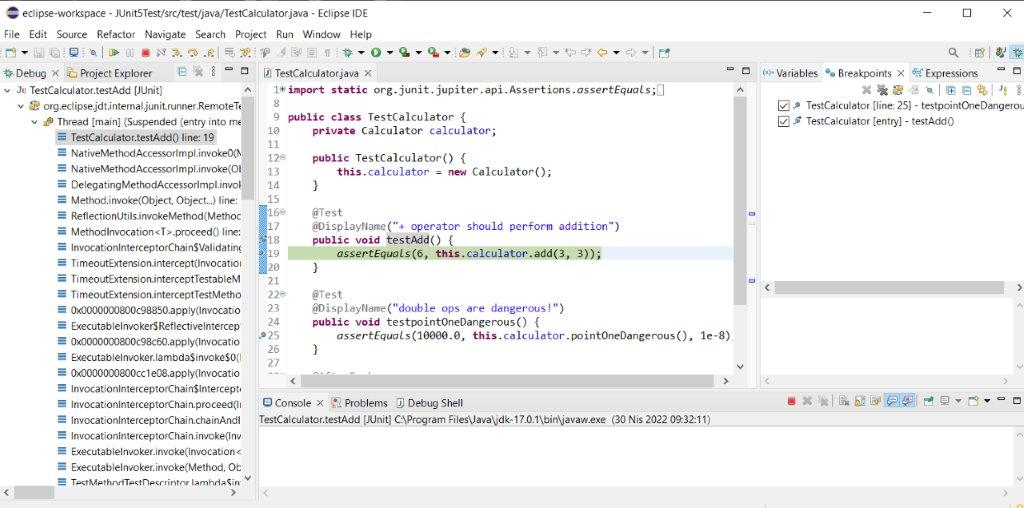
\includegraphics{images/eclipse-debugger-screenshot.jpg}
    \caption{A screenshot of Eclipse Debugger.}
    \labfig{fig:eclipse-debugger}
\end{figure}

\section{Unit Test Automation}
Unit tests can be performed manually or with the help of automation tools. JUnit (Java), TestNG (Java), NUnit (.net languages), Jasmine (Javascript), Html Unit (HTML), and Simple Test (PHP) are among the most popular open source unit testing tools and frameworks. In the second part of this book, JUnit tool will be introduced within the Eclipse Java IDE.  

\section{Problems}
\begin{enumerate}
    \item Create a new code review checklist, by modifying the one given in this chapter to facilitate its use for units (functions, procedures, methods, or modules). 
    \item Write a recursive C program to sort n numbers by the Quicksort algorithm. Create value, decision and statement mutants, and test cases. Compute the mutation score based on your test cases.  
    \item Explain the difference between static and dynamic unit testing.
    \item What is regression testing? At what levels of testing it is utilized?
    \item In debugging, what is a breakpoint (toggle point) in a program segment?
    \item Use Dev-C++ IDE to debug the prime number generation program given in this chapter to learn the debugging process. Insert breakpoints (toggle points), and use add watch facility to trace the execution.
    \item Repeat the same using an Eclipse IDE for C programming language.
\end{enumerate}